%%%%%%%%%%%%%%%%%%%%%%%%%%%%%%%%%%%%%%%%
% Classe do documento
%%%%%%%%%%%%%%%%%%%%%%%%%%%%%%%%%%%%%%%%

% Nós usamos a classe "unb-cic".  Deixe apenas uma das linhas
% abaixo não-comentada, dependendo se você for do bacharelado ou
% da licenciatura.

%\documentclass[bacharelado]{unb-cic}
\documentclass[licenciatura]{unb-cic}



%%%%%%%%%%%%%%%%%%%%%%%%%%%%%%%%%%%%%%%%
% Pacotes importados
%%%%%%%%%%%%%%%%%%%%%%%%%%%%%%%%%%%%%%%%

\usepackage[brazil,american]{babel}
\usepackage[T1]{fontenc}
\usepackage{indentfirst}
\usepackage{natbib}
\usepackage{xcolor,graphicx,url}
\usepackage[utf8]{inputenc}



%%%%%%%%%%%%%%%%%%%%%%%%%%%%%%%%%%%%%%%%
% Cores dos links
%%%%%%%%%%%%%%%%%%%%%%%%%%%%%%%%%%%%%%%%

% Veja o arquivos cores.tex se quiser ver que outras cores estão
% pré-definidas.  Utilizando o comando \hypersetup abaixo nós
% evitamos aquelas caixas vermelhas feias em volta dos links.

%%%%%%%%%%%%%%%%%%%%%%%%%%%%%%%%%%%%%%%%
% Cores do estilo Tango
%%%%%%%%%%%%%%%%%%%%%%%%%%%%%%%%%%%%%%%%

\definecolor{LightButter}{rgb}{0.98,0.91,0.31}
\definecolor{LightOrange}{rgb}{0.98,0.68,0.24}
\definecolor{LightChocolate}{rgb}{0.91,0.72,0.43}
\definecolor{LightChameleon}{rgb}{0.54,0.88,0.20}
\definecolor{LightSkyBlue}{rgb}{0.45,0.62,0.81}
\definecolor{LightPlum}{rgb}{0.68,0.50,0.66}
\definecolor{LightScarletRed}{rgb}{0.93,0.16,0.16}
\definecolor{Butter}{rgb}{0.93,0.86,0.25}
\definecolor{Orange}{rgb}{0.96,0.47,0.00}
\definecolor{Chocolate}{rgb}{0.75,0.49,0.07}
\definecolor{Chameleon}{rgb}{0.45,0.82,0.09}
\definecolor{SkyBlue}{rgb}{0.20,0.39,0.64}
\definecolor{Plum}{rgb}{0.46,0.31,0.48}
\definecolor{ScarletRed}{rgb}{0.80,0.00,0.00}
\definecolor{DarkButter}{rgb}{0.77,0.62,0.00}
\definecolor{DarkOrange}{rgb}{0.80,0.36,0.00}
\definecolor{DarkChocolate}{rgb}{0.56,0.35,0.01}
\definecolor{DarkChameleon}{rgb}{0.30,0.60,0.02}
\definecolor{DarkSkyBlue}{rgb}{0.12,0.29,0.53}
\definecolor{DarkPlum}{rgb}{0.36,0.21,0.40}
\definecolor{DarkScarletRed}{rgb}{0.64,0.00,0.00}
\definecolor{Aluminium1}{rgb}{0.93,0.93,0.92}
\definecolor{Aluminium2}{rgb}{0.82,0.84,0.81}
\definecolor{Aluminium3}{rgb}{0.73,0.74,0.71}
\definecolor{Aluminium4}{rgb}{0.53,0.54,0.52}
\definecolor{Aluminium5}{rgb}{0.33,0.34,0.32}
\definecolor{Aluminium6}{rgb}{0.18,0.20,0.21}

\hypersetup{
  colorlinks=true,
  linkcolor=DarkScarletRed,
  citecolor=DarkScarletRed,
  filecolor=DarkScarletRed,
  urlcolor= DarkScarletRed
}



%%%%%%%%%%%%%%%%%%%%%%%%%%%%%%%%%%%%%%%%
% Informações sobre a monografia
%%%%%%%%%%%%%%%%%%%%%%%%%%%%%%%%%%%%%%%%

\title{Criação de um Framework para aplicação de Ética em Inteligência Artificial}

\orientador{\profa \dra Edna Canedo}{CIC/UnB}
%\coorientador[a]{\prof[a] \dr[a] Coorientadora}{MAT/UnB}
\coordenador{\prof \dr Pedro Rezende}{CIC/UnB}
\diamesano{15}{fevereiro}{2021}

\membrobanca{\prof \dr Professor I}{CIC/UnB}
\membrobanca{\prof \dr Professor II}{CIC/UnB}

\autor{Anayran Pinheiro de }{Azevedo}
\CDU{004.4}

\palavraschave{Inteligência Artificial, Controle, Qualidade, Responsabilidade, Ensino, Educação, EAD, Software, Agile }
\keywords{Artificial Intelligence, Control, Quality, Responsibility, Teach, Education, Remote Teaching, Software, Agile}



%%%%%%%%%%%%%%%%%%%%%%%%%%%%%%%%%%%%%%%%
% Texto
%%%%%%%%%%%%%%%%%%%%%%%%%%%%%%%%%%%%%%%%

\begin{document}
  \maketitle
  \pretextual

  \begin{dedicatoria}
  Dedico a....
  \end{dedicatoria}

  \begin{agradecimentos}
  Agradeço a....
  \end{agradecimentos}

  \begin{resumo}
  Em um mundo onde os avanços tecnológicos são tão rápidos, a tomada de decisão para uma ágil implantação e/ou adaptação se torna também necessária, levando a criação de várias metodologias que vão auxiliar desde a idealização, passando pelo planejamento e implantação até a finalização destes projetos que foram pensados. Com este desafio se aplicando a todo o mundo, não seria impensável que mesmo no ramo de Inteligência Artificial este modelo de desenvolvimento ágil também estivesse incluso. Porém, também junto com este desenvolvimento, vemos a necessidade de pensar nas implicações éticas do uso de tal tecnologia, que traz consigo importantes desafios a serem superados. Neste trabalho, veremos como a aplicação da metodologia ágil impactou na criação de um framework para auxílio dos desenvolvedores e usuários da tecnologia a facilitar o debate e implantação de princípios éticos de IA em seus trabalhos, também como foi o desenvolvimento da ferramenta e seu uso devido, gerando assim um impacto imediato para os potenciais usuários e possibilidades de melhoras futuras, tanto nos projetos futuros quanto no projeto da própria ferramenta. 
  \end{resumo}

  \selectlanguage{brazil}
  \begin{abstract}
  The science...
  \end{abstract}
  \selectlanguage{brazil}

  \tableofcontents
  \listoffigures
  \listoftables

  \textual
  \chapter{Introdução}

\section{O que é Inteligência Artificial? E o que é a aplicação da ética em Inteligência Artificial?}

	
\begin{figure}
            \begin{center}
                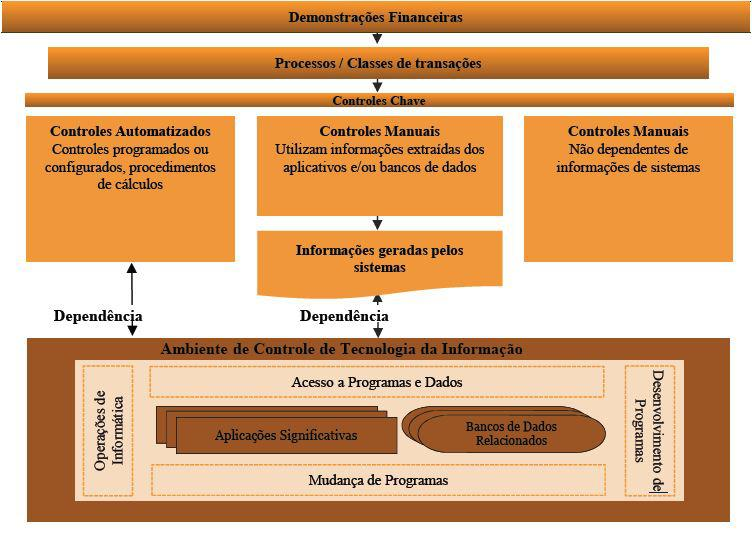
\includegraphics[width=0.7\textwidth]{Img1}
            \end{center}
            \caption{Como o ambiente de TI suporta as operações financeiras de um negócio hoje em dia.}
            \label{fig:Img1}
\end{figure}

\section{Inteligência Artificial}

    Lorem Ipsum Dolor Sit Amet\cite{SOX}
	
\subsection{Ética}

	Blablabla

\begin{itemize}
\item    Financeira (segundo a visão dos acionistas);
\item	 Cliente;
\item	 Processos internos de negócios;
\item	 Inovações.
\end{itemize}

Ao nos mostrar através de tais visões o que é mais crítico, esta framework permite direcionar recursos para os processos que adicionarão valor à empresa, de fato. A tecnologia entra nesta metodologia como uma valiosa peça para colocar o BSC em funcionamento, porém não como peça suficiente pelo fato desta ferramenta administrativa interagir com a cultura da corporação. Devido à sua grande complexidade e por envolver a estrutura empresarial como um todo, a adoção deste modelo deve partir da alta direção ou, a depender do caso, do presidente da empresa para que sua implementação seja viável.

Por ser um modelo razoavelmente flexível, permite ajustes temporários para se adequar ao objetivo final, que é a valorização da empresa. Esta visão ainda nos permite:

\begin{itemize}
\item Perspectivas diferentes da visão dos negócios;
\item Uma melhor monitoração e elaboração das estratégias;
\item Análise das relações de causa e efeito a partir de um macro indicador;
\item Alinhamento e compartilhamento da visão e metas desde o nível estratégico, passando pelo tático até alcançar o nível operacional;
\item Uma definição mais efetiva dos planos de ações;
\item Maior acurácia dos planos de ações a serem tomadas;
\item Maior eficiência do tempo a ser usado no processo de decisão
\item Colaboratividade através de mecanismos de compartilhamento de informações analíticas
\end{itemize}

Com a metodologia BSC como opção de gestão na Governança em TI, podemos realizar uma melhor avaliação e obter uma melhor gestão da organização não apenas de forma limitada apenas às medidas tradicionais de resultados e desempenho financeiros, mas também complementá-la com medidas de outras dimensões como a atenção na satisfação dos clientes, satisfação nos controles internos e capacidade de inovação e aprendizado. Tais dimensões adicionais nos garantem, se integradas, melhores resultados futuros e não apenas uma visão meramente dos resultados passados, obtidos apenas em uma perspectiva de gestão puramente financeira, mas também valorizando o capital que executa este serviço, seja ele humano ou seja ele automatizado.

\subsection{COBIT}

Criado em 1996 nos Estados Unidos, a metodologia COBIT (Control Objectives For Information and related Technology) foi criada pelo Information System Audit and Control Association (ISACA) com a intenção de ser um guia de boas práticas apresentado como um framework a partir de ferramentas de auditoria, funcionando como um um norte para a gestão da TI nas empresas, literalmente.

Esta metodologia apresenta padrões independentes, podendo ser implementada por qualquer tipo de negócio, com qualquer tipo de valor e de participação da tecnologia da informação dentro de sua cadeia produtiva. No momento, a versão utilizada do COBIT é a versão 5. Sua integração com outras frameworks foi ampliada com a intenção de aumentar a agregação entre estas ferramentas e, assim, possibilitar uma melhor produtividade. As frameworks que trabalham em conjunto com tal framework são em sua maior parte o ITIL, ISO, PMBOK (Projetct Management Body of Knowledge) e o TOGAF (The Open Group Architecture Framework).\cite{COBIT-4.1} \cite{SOX-COBIT}
	


        \begin{figure}
            \begin{center}
                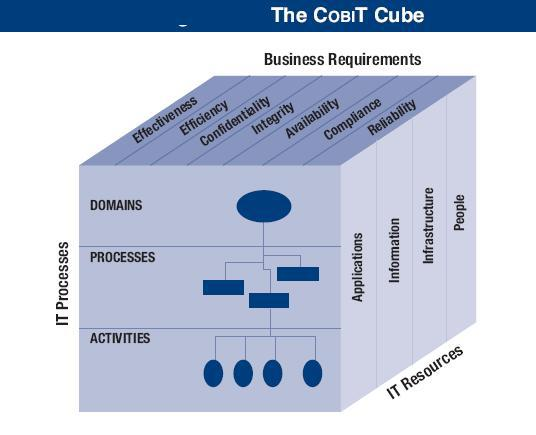
\includegraphics[width=0.7\textwidth]{Img2}
            \end{center}
            \caption{Cubo de aplicação do COBIT, mostrando seus processos, recursos e requisitos de negócios e sua abrangência. (COBIT 5, apud https://jane15cl.wordpress.com/2011/01/)}
            \label{fig:Img2}
        \end{figure}



Com o exame e aplicação do COBIT conforme as necessidades do negócio, este framework começou a ser extensivamente utilizado pelos auditores e gerentes por ser uma ferramenta que apresenta uma grande abrangência dos controles, porém de forma reduzida para que se possa visar uma melhor abrangência do ambiente a ser verificado.

Esta metodologia é voltada para três níveis distintos:
\begin{itemize}
    \item Gerentes que necessitam avaliar os riscos e controlar os investimentos de TI;
    \item Usuários que necessitam assegurar a qualidade dos serviços prestados para seus clientes, sejam estes internos ou externos;
    \item Auditores que precisam avaliar o trabalho da gestão de TI e aconselhar o controle interno da organização.
\end{itemize}

O principal foco é apontar onde possíveis melhorias devem ser realizadas e, nos casos em que seja necessário o exame, se possibilite o desenvolvimento e a implementação de novos procedimentos e controles.  Desta forma, uma política de revisão constante com o objetivo de manter a eficácia dos mesmos é essencial.

Podemos aqui apresentar algumas recomendações sobre os controles:
\begin{itemize}
    \item Os controles devem ser os mais simples e objetivos possíveis;
    \item As atualizações de revisões devem ser devidamente documentadas e armazenadas;
    \item O processo de revisão deve perturbar o mínimo possível as funções de rotina, ou seja, a revisão de tal processo não deve gerar um grande impacto no negócio de forma a diminuir sua eficiência;
    \item O processo de revisão deve ser automatizado e suas atualizações produzidas sistematicamente, de preferência;
    \item A frequência da revisão dos itens de controle se dá de acordo com a conformidade e a necessidade do negócio, podendo ser semanal, mensal, trimestral, etc.
\end{itemize}
\subsection{ITIL}	
	\cite{ITIL-OVERVIEW}

	Criado no final dos anos 1980 pela Central Computing and Telecommunications Agency, hoje Office for Government Commerce para o governo britânico, o ITIL (Information Technology Infrastructure Library) reúne um conjunto de recomendações, sendo dividido em dois blocos que por sua vez se subdividem-se em cinco outros blocos:
 
Entrega de serviço, que engloba os tópicos de gerenciamento de níveis de serviço, gerenciamento de capacidade, gerenciamento de finanças, gerenciamento de disponibilidade e continuidade de serviço e;


Suporte de serviços, que engloba o service desk, o gerenciamento de incidentes, o gerenciamento de problemas, o gerenciamento de configurações, o gerenciamento de mudanças e o gerenciamento de versões.

	Por sua grande flexibilidade, a adoção do ITIL traz grandes benefícios, uma vez que ele não define quais processos devem ser implementados, mas sim mostra quais são as melhores práticas a ser utilizadas. De forma clara, podemos mostrar alguns resultados decorrentes de sua implementação, tais como:

Definição dos ciclos de vida dos processos;
Análise e classificação dos erros;
Aumento no grau de segurança do usuário;
Organização de métodos de trabalho;
Geração de contínuas melhorias e referências para novos usuários;
Contribuição como facilitador e integrador entre as áreas de trabalho;
Disponibilização dos recursos tecnológicos em tempo integral;
Restauração da operação normal do serviço;
Avaliação de impactos de mudança;
Obtenção e uso de indicadores;
Entre outros.

	Complementar ao COBIT, o ITIL é uma série de documentos usada como auxílio à implementação de uma estrutura de gerenciamento de serviços de TI, uma biblioteca que descreve detalhadamente as melhores práticas de gestão, elaboradas especificamente para a área de TI. Os pontos focados apresentam as melhores práticas para a central de atendimento, para o gerenciamento de incidentes, para o gerenciamento de problemas e também para o gerenciamento financeiro para serviços de TI, com a finalidade de ajudar no objetivo de definição do gerenciamento de serviços e suas aplicações para empresas especificas, independente do aplicativo ou plataforma e, sendo assim, aplicável a qualquer empresa.

\subsection{CMMI}

	CMMI é um modelo de referência que possui práticas necessárias à maturidade em disciplinas específicas, podendo estas ser genéricas ou específicas. Ele se destina a auxiliar empresas a melhorar a produtividade dos processos de desenvolvimento de software e a organizar o funcionamento dos ambientes de tecnologia de informação. Esta metodologia ajuda a mostrar quais metas devem ser alcançadas através da quantificação, orientação e qualificação dos estágios de maturidade da empresa.
	O CMMI é definido em quatro níveis de maturidade para os ambientes de desenvolvimento de software (incompleto, inicial, repetível e definido), sendo cada um destes composto por um conjunto de áreas-chave de processos que descrevem as questões e os grandes temas que devem ser abordados e resolvidos para o alcance de um determinado nível de maturidade definido segundo o framework. 
	\cite{CMMI}
	
\section{Processos utilizados na auditoria de sistemas}
	
	Quando a Tecnologia da Informação é usada para iniciar, gravar, processar e reportar transações ou outros dados financeiros para a sua inclusão nos relatórios financeiros, devemos considerar como tais informações (e seu gerenciamento, caso sejam relevantes), estão mapeadas, bem como se estão de acordo com os processos de negócios (incluindo o processo da demonstração financeira em si), com os sistemas e ambientes computacionais para cada unidade de gerenciamento significante, seu entendimento e avaliação. Desta forma, verifica-se:
\begin{itemize}
    \item As principais características dos sistemas e ambientes;
    \item Gerenciamento dos sistemas de informações e tecnologia;
    \item Mudanças de sistemas e ambientes significantes que podem impactar na geração do relatório financeiro;
    \item Problemas reconhecidos dos sistemas;
    \item Como a instituição tem respondido aos riscos de distorções materiais que podem surgir dos sistemas de informação e tecnologia.
\end{itemize}


	Ao se analisar tais aspectos, se fazem necessárias a avaliação dos controles da área da tecnologia, da eficiência dos sistemas de informação, e a verificação e cumprimento das legislações e normativos aos quais estão sujeitos e da gestão eficaz dos recursos de informática. Para a análise destes processos, quatro atividades são realizadas, quais sejam: a verificação de acessos a programas e dados, o desenvolvimento dos programas utilizados pela empresa, a gerência de mudanças e as operações de informática, as quais descreveremos logo a seguir.	

\subsection{Acesso a Programas e Dados}

	Este elemento agrupa controles relacionados ao gerenciamento de acesso a sistema e dados, tanto lógicos quanto físicos. O foco destes controles é a redução de risco de acesso inapropriado ou não autorizado a sistemas de informações e a prevenção da execução ou ocultação de erros ou irregularidades. As áreas de controle relevantes a este elemento incluem:
\begin{itemize}
\item    \subsubsection{Políticas de TI}
	Uma política de segurança formalizada tem sido adotada, a qual é revisada e aprovada pela gerência. A política deve ser comunicada a todos na organização.
\item	\subsubsection{Data Center}
	O acesso físico ao Data Center é restrito ao pessoal apropriado.
\item	\subsubsection{Parâmetros de senhas}
	Os parâmetros de senhas da rede estão apropriadamente configurados, assim como para os sistemas críticos e sua relevante infraestrutura (como banco de dados e sistemas operacionais).
\item	\subsubsection{Contas superusuários (root)}
	Acessos a contas root ou privilegiadas da rede, sistemas críticos, sistemas operacionais e banco de dados são restritos a um determinado grupo de adminstradores de sistemas.
\item	\subsubsection{Provisão ou modificação de acesso ao usuário}
	Existem procedimentos predefinidos para outorgar ou modificar acessos e direitos de acesso para usuários em sistemas relevantes ao negócio. Tais procedimentos exigem uma aprovação formal para a garantia ou modificação destes.
\item	\subsubsection{Retirada de acesso}
	Existem procedimentos para a restrição do acesso e seus direitos aos usuários para os sistemas relevantes. A revogação destes acessos é realizada de forma eficiente e em tempo hábil.
\item	\subsubsection{Revisões periódicas de acesso a usuários}
	Revisões periódicas são executadas de forma a identificar se os usuários ativos estão com seus devidos acessos e, caso não estejam, adequá-los de acordo com as políticas internas da empresa, limitando o acesso à rede, aos sistemas e à infraestrutura.
\end{itemize}
\subsection{Desenvolvimento de Programas}
	Este elemento é relevante para os controles de desenvolvimento de novas aplicações ou sistemas. O objetivo destes controles é garantir que novos sistemas que são desenvolvidos ou adquiridos sejam autorizados, testados, aprovados, devidamente implementados e documentados.
	
\begin{itemize}
\item	\subsubsection{Metodologias}
	O ciclo de vida do desenvolvimento de sistemas segue uma metodologia para a aquisição ou desenvolvimento de novos sistemas ou aplicações. De maneira similar ao gerenciamento de mudança de programas, todas as novas aquisições ou desenvolvimentos são aprovados, testados e documentados.
\end{itemize}

\subsection{Mudança de Programas}

	Este elemento é relevante para os controles de mudança de aplicações ou de sistemas. O objetivo destes controles é garantir que novas versões desenvolvidas ou adquiridas sejam autorizadas, testadas, aprovadas, devidamente implementadas e documentadas.
\begin{itemize}
\item	\subsubsection{Gerenciamento de mudança de programas}
	As mudanças realizadas nos sistemas seguem políticas de gerenciamento de mudanças e procedimentos estabelecidas pela gerência (inclusive mudanças de configurações ou mudanças emergenciais). Estas mudanças são registradas, aprovadas e testadas antes de serem promovidas para o ambiente de produção.
	
\item	\subsubsection{Segregação de cargos}
	Deve ser garantida uma segregação de cargos entre os desenvolvedores, os homologadores e o ambiente de produção, sendo tolerável que o desenvolvedor ou o usuário final possa ser também um homologador.
\end{itemize}
\subsection{Operações de Informática}

	Este elemento agrupa os controles ligados a assuntos operacionais, como backups e procedimentos em batch (procedimentos em lote).  O objetivo destes controles é garantir que o processamento do sistema ou aplicação esteja apropriadamente autorizado e agendado, e que as variações de agendamento sejam identificadas e resolvidas. As áreas de controles relevantes a este elemento incluem:
    
\begin{itemize}
\item	\subsubsection{ Processamento/Monitoramento de trabalhos em batch}

	Os procedimentos de monitoramento são desenvolvidos para prover garantias razoáveis em relação à completude e à oportunidade do processamento de dados no sistema.

\item	\subsubsection{Gerenciamento de incidentes}

	A organização tem processos para gerenciamento de incidentes para tratar incidentes de prioridade média ou alta dentro de um prazo preestabelecido.
	
\item	\subsubsection{Backup de sistemas}
	
	As rotinas de backup e recuperação são implementadas pela gerência de modo a garantir que os dados, transações e programas necessários para a geração dos relatórios financeiros possam ser devidamente recuperados. Os procedimentos de backup e restore são testados periodicamente.
	
\item	\subsubsection{Armazenamento remoto}
	
	Procedimentos devem ser estabelecidos para armazenar o backup em um estabelecimento remoto (podendo este ser de terceiros ou não) de maneira periódica. O acesso a estes locais é gerenciado de forma restrita para pessoas autorizadas segundo as responsabilidades profissionais.
\end{itemize}

O processo de auditoria visa garantir a qualidade dos sistemas e serviços e consequentemente a confiabilidade das instituições auditadas. O alto custo deste processo requer atenção à otimização do mesmo. A correta aplicação da engenharia de software permite não só maior confiabilidade dos sistemas gerados, facilitando o processo de auditoria, como também procura atestar uma melhor compreensão do sistema auditado, seja pela presença de documentação relevante, seja pela correta estruturação daquele. Estas qualidades permitem também maior facilidade de atualização ou alteração do sistema, tornando mais eficiente a adequação do mesmo a padrões de qualidade ainda não respeitados e à correção de erros identificados ao longo do processo de auditoria.
	
Mas como esta breve introdução pode ter a ver com a educação nas instituições? Será que podemos nos permitir questionar que tais métodos podem não somente ajudar a instituição a ter ganhos em eficiência, mas não somente no quesito sistêmico? Ora, muitas vezes vemos várias empresas e instituições (afinal a governança não deve servir apenas para o mercado financeiro, na visão de lucros) implantarem políticas organizacionais, e até mesmo políticas focadas para que a TI seja, de fato, o suporte do negócio. 

Mas como tem sido a aplicação destas políticas para os funcionários? Eles tem aceito isto de forma unilateral, únicamente pela necessidade de se manter no trabalho? A empresa tem visto tal problema também da ótica do "chão de fábrica"? Pois sempre é válido pensarmos que se temos ferramentas que podem servir para aumentar nossos ganhos, usá-la a nosso favor. Porém será que elas são suficientes por si só, sem nenhum processo de ensino e aprendizagem para não somente começar o trabalho, mas principalmente mantê-lo e ajudar a empresa a atacar problemas que podem ser não somente de cunho estrutural da mudança em si, mas também da mentalidade das pessoas que adentram ao negócio?

Este serão alguns dos questionamentos que vamos tentar esclarecer ao longo do nosso trabalho. Porém antes, para tanto iremos passar por alguns tópicos para nos ajudar a melhor estruturar nosso trabalho. Teremos que primeiro conhecer um pouco mais a fundo o que é a governança em TI, quais são os processos que supostamente precisam acompanhar para a correta implantação do sistema e das novas políticas, quais ferramentas educacionais poderão nos ajudar durante estes processos e se eles são suficientes. Vamos acompanhar também um estudo de caso de gestão de mudança e como uma ferramenta educacional ajudou durante este processo. 

Veremos também ao longo deste trabalho, como estes casos são mais comuns na literatura do que imaginamos (tanto quanto da nossa parte não termos tido facilidades em achar trabalhos produzidos no país sobre esta área) e quais foram as soluções encontradas. Esperamos ao final deste trabalho esclarecer como a educação tem a ver com a governança em TI, e como a informática pode fornecer um valioso suporte para tais políticas que iremos estudar.
  \chapter{A importância da governança TI para o cenário profissional}
\section{A importância da governança TI para o cenário profissional}
É inegável que temos desde os primórdios da mistura entre negócios e tecnologia da informação uma certa preocupação em analisar e quantificar como não somente a adequação do sistema tem ocorrido, mas também se os recursos humanos o qual usufrirão de tais sistemas estão fazendo-o corretamente. Verificar se tais investimentos de finanças e esforços acadêmicos estão retornando resultados é algo essencial, porém mesmo com uma abundante quantidade de estudos que vemos saindo dia após dia, ainda pairam dúvidas se de fato temos como quantificar e qualificar este esforço. Somente assim podemos ter dados de tais métricas e como os problemas possam ser mapeados e corrigidos, qualidades possam ser aprimoradas e verificar "pontos vazios" para a criação ou inserção de novas técnicas.  Porém, como o autor abaixo explica:
\begin{quotation}

    "Enquanto grandes investimentos vêm ocorrendo na área de informática, muito pouco se sabe sobre seus efeitos nas organizações, especialmente porque o relacionamento entre a TI e o desempenho organizacional tem se mostrado bastante complexo e multifacetado, dificultando a identificação e a avaliação do impacto financeiro destes investimentos. Willcocks e Lester (apud LIN; PERVAN, 2001\cite{LIN}) apontam três justificativas pelas quais a identificação e a avaliação do impacto organizacional da TI são prejudicadas. São elas: (a) muitos executivos acreditam que não existe uma solução viável para esse problema, pois por razões competitivas percebem que não podem deixar de investir em TI, mesmo que não encontrem uma justificativa economicamente plausível; além disso, (b) como a infra-estrutura de TI se torna uma parte inseparável dos processos e da estrutura da organização, torna-se difícil separar o impacto proporcionado pela TI das demais atividades da organização; e (c) a existência de uma lacuna na identificação e compreensão dos custos, benefícios e riscos envolvidos nas diferentes tecnologias adotadas que dificulta a visualização do retorno de cada uma delas."(LUNARDI; 2008)\cite{ESTUDO-EMPIRICO}


\end{quotation}    
    
É explícito que o investimento somente na área de tecnologia não é a solução definitiva de tais problemas, visto que mesmo com a proposta de tentar facilitar processos e procedimentos ainda é fortemente dependente de humanos responśaveis pela execução destes processos. Verificar como se ocorrerá a gestão de mudança, tanto pela parte comportamental quanto pela parte da cultura da empresa, não somente para que o uso da ferramenta possa ser eficiente, porém principalmente para que o investimento realizado em tais ferramentas de suporte façam sentido ao gasto demandado por tal problema. O uso das ferramentas de TI por si só não é capaz sozinha de aumentar os ganhos da produtividade, seu correto uso sim. Não somente pela organização, como um todo, mas principalmente de forma nuclear, no funcionário que realiza o trabalho considerado como "chão de fábrica", onde ele será o operador final de tal ferramenta. Este funcionário, que é o motivo da empresa prosperar e manter seu nome como um todo, se não for corretamente condicionado ao uso de tal ferramenta, pode ser o início de uma corrente extremamente desastrosa, em especial no aspecto financeiro. E é neste aspecto onde mora o diferencial entre empresas e empresas, onde com o uso da mesma ferramenta de suporte, ela é capaz de obter extremos ganhos ou perdas, determinando o sucesso não somente comercial mas também até mesmo o nome e tradição da empresa, caso esta já possua uma.

A habilidade - ou a ausência de tal - tem sido o principal determinante para o posicionamento estratégico de diversas empresas, seja para o sucesso ou para o fracasso. (apud WEILL; OLSON\cite{WEILL}) Tal conceito é chamado de {\bf efetividade de conversão} segundo os autores Peter Weill e Margarethe Olson, em março de 1989 (mostrando a nós como tal conceito tem mais tempo do que imaginávamos). A partir deste ponto de vista, diversos pesquisadores ao redor do globo tem pesquisado e procurado propor modelos teóricos para analisar como os investimentos, que tanto foram citados nas páginas anteriores, podem criar valor para os negócios, aumentar a produtividade ou, até mesmo, ampliar o desempenho organizacional. A partir desta ótica, é possível verificação entre o sucesso e o fracasso no valor gerado pela TI para o seu foco de serviço, determinando até que ponto esta área funcionou como uma catalisadora para seus negócios e, assim, trazer capacidade de organização de gerência e potencialilzação de investimentos.

\section{Governança em TI, de onde veio?}
Por curiosidade, o termo {\bf Governança em TI} surge como uma tentativa de garantir a agregação de valor aos negócios da organização após investimentos realizados em tecnologia (apud DE HAES; VAN GREMBERGEN, 2005)\cite{DEHAES2005}. Desta forma, verificamos que a governança de TI gera um efeito direto sobre a gestão da TI, visto onde é através dela que um conjunto de regras são criadas, definidas, postas em ação e avaliadas para governar toda a função da TI na organização (apud VERHOEF, 2007 \cite{VERHOEFF}).

Tal metodologia começou a ser largamente adotada após no final dos anos 90, com a quebra de grandes empresas americanas, decorrente de fraudes em seus relatórios financeiros, onde em um cenário em que a governança corporativa e responsabilidade fiscal passaram a ter um grande interesse no meio empresarial, apoiado por um meio de justificar e, principalmente, dar mais efetividade nos investimentos realizados nesta área.

Usando as palavras do autor Guilherme Lerch:
\begin{quotation}
\textit{"A governança de TI, propriamente dita, envolve a aplicação de princípios de
Governança Corporativa para dirigir e controlar a TI de forma estratégica, preocupando-se
exclusivamente com dois assuntos-chave: o valor que a TI proporciona à organização, e o
controle e a diminuição dos riscos relacionados à TI (ITGI, 2003\cite{ITGI}; PETERSON, 2004b\cite{PETERSON}; HARDY, 2006\cite{HARDY}). O primeiro assunto é direcionado pelo alinhamento estratégico entre os negócios e a tecnologia, enquanto que o segundo é direcionado pela definição dos responsáveis na organização pelas decisões envolvendo os assuntos ligados à TI. Para que isso ocorra, é necessário que os recursos tecnológicos da organização sejam adequados e que o seu desempenho seja constantemente mensurado (ITGI, 2003\cite{ITGI})."}
\end{quotation}

Ora, é possível notarmos aqui que a governança da TI vai muito além do que a gestão da TI, vemos como todas as questões da organização, sejam quaisfor, estão sendo suportadas e relacionadas diretamente pela tecnologia, desde a definição dos direitos e responsabilidades sobre a área, passando pelo estudo e aprovação dos de investimentos tecnológicos para as melhorias do negócio, pelo monitoramento e manutenção da TI já presente no local, até chegar na avaliação do valor dado pelo departamento ao negócio. Daí, o fator da \textbf{efetividade de conversão da TI} neste caso não é ligado apenas a delegação do uso da tecnologia pela empresa, porém juntamente, as decisões que são antecedidas da sua aquisição, bem como o valor que o uso desta ferramenta pode impactar a organização.

Logo, não é incomum vermos que empresas que dispõem de tal política como algo inerente à cultura e organização possuem uma vantagem, tanto financeira quanto organizacional, para estarem se aproximando de uma posição privilegiada no mercado, se não a posição de destaque a depender do mercado o qual atua e de sua gerência, visto que a aplicação dos mesmos {\it frameworks} podem gerar distintos resultados a depender da empresa e sua cultura, organização e até mesmo processo de implantação.

\section{Cultura organizacional e gestão de mudança}

Para entendermos um pouco melhor, vamos explorar como e o que é a cultura organizacional de uma empresa. Segundo o texto retirado do site portal-administração, o conceito é:

\begin{quotation}
...a cultura organizacional é um conjunto de hábitos, crenças e valores, que por sua vez, são estabelecidos através de normas, princípios, atitudes e perspectivas compartilhadas pelos colaboradores de uma empresa. Basicamente, ela constitui o modo de pensar e agir da companhia (sendo um dos principais fatores que diferencia uma empresa das demais). Podemos dizer também que a essência da cultura de uma empresa é a própria maneira como a mesma realiza seus negócios, lida com seus clientes e colaboradores e o grau de lealdade que eles transmitem para com a organização.(PORTAL DA ADMINISTRAÇÃO, 2014)\cite{PORTALADM}
\end{quotation}

O esclarecimento do conceito acima nos ajuda a começar a entender como e por onde podemos começar o desenvolvimento de uma política de governança em TI. Para tanto, façamos o seguinte exercício. Vamos imaginar uma grande empresa onde, tradicionalmente, boa parte de seus processos de negócios eram feitos através de processos manuais. Desde a aferição de balanços até a contagem de estoques, passando pelo registro de folhas de ponto. Nós, como estudantes da área de tecnologia logo imaginamos porque não há um sistema que pode gerenciar tudo isto (afinal, tais sistemas existem já faz muitos anos). 

Porém após realizarmos que antes da governança, devemos nos lembrar da gestão, já começamos a imaginar onde podem ser os possíveis gargalos. O primeiro já identificado por inferência ao longo do texto é de como esta gestão de mudança deverá agir em conformidade com a cultura organizacional da empresa. Por mais que a empresa e seus colaboradores compartilhem de um determinado comportamento, uma gestão de mudança sempre pode ser fortemente afetada caso não esteja em harmonia com o momento da empresa, preparação dos colaboradores, preparação do ambiente, capacidade financeira para tal e, principalmente, se a empresa se encontra no momento certo para tal coisa. 

E para corroborar como o momento certo pode influênciar, de acordo com o professor Reinaldo Lucas:
\begin{quotation}
"...tudo na vida funciona dentro de um ciclo, que é chamado ciclo da evolução dos organismos. Este ciclo tem cinco etapas: formação, tumulto, normalidade, desempenho e acomodação. Qual é o tempo deste ciclo? É muito relativo. Dizem que na vida dos indivíduos é em torno de sete anos. Há estudos que mostram que as empresas no Brasil morrem depois do terceiro ciclo. Então, é importante percebermos qual é o momento em que a empresa começou a se acomodar e aí fazer uma mudança. Esta mudança normalmente tem que envolver a sua estratégia, a sua estrutura, os seus processos e as pessoas. Então, qual é o momento ideal para mudar? É o momento em que a empresa começou a acomodar, mas também não se pode ter um processo constante de mudança porque a mudança constante destrói a empresa. É preciso ter sempre períodos de evolução e períodos de revolução. A medição acontece muito em função do tipo de negócio. Se pegarmos uma indústria de telefone celular, essa mudança é muito acelerada pela tecnologia. Se pegarmos uma mineradora, o tempo entre uma mudança e outra é muito maior. Então, depende muito do segmento de negócio."\cite{FDC}
\end{quotation}

Porém, para melhor compreendermos tal questionamento, o que é uma mudança dentro deste contexto? Segundo Chiavenato:

\begin{quotation}
Mudança é a transição de uma situação para outra diferente ou passagem de um estado
para outro diferente. Mudança implica ruptura, transformação, perturbação,
interrupção. O mundo atual se caracteriza por um ambiente dinâmico em constante
mudança e que exige das organizações uma elevada capacidade de adaptação, como
condição básica de sobrevivência. Adaptação, renovação e revitalização significam
mudança.\cite{CHIAVENATO}
\end{quotation}

É nestas horas que paramos para pensar e perceber como a implantação de uma política de governança pode ser mais difícil do que se imagina. Ter que pensar em todos os tópicos acima citados, além de realizar a gestão pré, durante e pós implementação de algo novo são processos penosos. Porém, ainda assim, temos casos de como uma correta gestão de mudança, aliada a uma forte política de governança em TI pode maximizar ganhos financeiros de empresas.

Um dos inúmeros cases que temos disponíveis para consulta foi realizado por dois professores, em que descrevem a implantação das métricas e políticas que vieram em conjunto com as práticas de governança em TI. Este cenário de estudo foi em uma empresa de telecom, a qual não tem seu nome divulgado por motivo não explicado no artigo apresentado. Esta empresa só veio adotar novas políticas de governança após uma mudança no setor de telecom após a criação da lei 9.472 (BRASIL, 1997)\cite{9472}.

O ponto levantado pelos pesquisadores Sortica e Graeml após a pesquisa pode ser lido de forma resumida abaixo:
\begin{quotation}
"O objetivo do estudo que motivou este artigo foi compreender a forma de utilização dos
critérios de efetividade da governança de TI (tecnologia da informação) na implementação de
estratégias por uma empresa fornecedora de serviços para o setor de telecomunicações. Para tanto, foram verificadas a existência e a utilização de critérios de efetividade tático-operacional, definidos nos modelos de governança tecnológica. 

A seguir, foi verificada a existência e a utilização
de critérios de efetividade estratégica, conforme apresentados na literatura. O estudo de caso
envolveu a realização de entrevistas semi-estruturadas, a partir das quais foram obtidos os dados para análise, em adição a dados documentais disponibilizados pela empresa. Observou-se que todos os critérios de efetividade tático-operacionais previstos nas categorias estudadas foram implementados na organização, embora se tenha verificado que algumas categorias de critérios de efetividade estratégica não estejam presentes ou não estejam completamente implementadas.

Detectou-se uma sobrevalorização de aspectos tático-operacionais da operação, quando contrastados com os aspectos estratégicos do negócio, o que é comum em empresas que têm processos produtivos complexos, que precisam ser bem gerenciados para que se garanta a qualidade do produto ou serviço oferecido ao mercado. \cite{Sortica}"
\end{quotation}

Mostrando o resultado com um ponto deste assunto, e um dos mais importantes, segue citação:
\begin{quotation}
"A governança tecnológica, como metodologia e parte fundamental da governança corporativa,
traz um conjunto de benefícios técnicos e operacionais à organização analisada e ao seu relacionamento
com as operadoras de telecomunicações (seus clientes). As prerrogativas da gestão,
como lucratividade e fidelidade aos investidores são dependentes de princípios estabelecidos para
a QoS (quality of service), como disponibilidade dos sistemas de informação, dependente da
criticidade do processo; interdependência dos processos; segurança da informação; e desempenho
dos serviços de TI por meio dos SLA."  \cite{Sortica}
\end{quotation}

Até aqui, temos um cenário ideal, um cenário onde o que se compõe são as metodologias, o maquinário, os {\it frameworks} e demais aspectos que servem de ferramentas, mas e como o material humano entra nesta área? Como será que a parte que pode colocar um negócio tanto em posição de destaque quanto levar à falência empresas tem agido perante tal cenário, que mesmo sendo estudado há mais de 20 anos, com testes e novas tecnologias surgindo a todo o momento para facilitar a adaptação da empresa e até mesmo do material humano envolvido, tem sido trabalhada? Será que o processo da implantação está passando somente por um processo puramente administrativo? Será que o processo de transmitir o que a empresa deseja a seu colaborador tem sido feito de uma forma efetiva? 

\section{Como a cultura organizacional e a governança em TI podem se relacionar}

Durante a pesquisa sobre como a cultura organizacional e a governança podem se relacionar, nos deparamos com uma pesquisa de três professores, onde abrem o seu artigo com a tese que é possível sim basear um modelo de governança de TI relacionando com o framework de Deter et al's (2000). Para tanto, primeiro foi necessário ligar seus métodos ao cenário de governança em TI. Como já vimos em partes como funciona a cultura organizacional de uma empresa, vamos listar abaixo os oito pontos que este framework possui.\cite{exploringit}

\subsection{Modelo de cultura organizacional Detert et al (2000)}
    \subsubsection{2.4.1.1. A base da verdade e da racionalidade}
    Se foca no grau onde cada colaborador acredita que algo é ou não real e como a verdade pode ser descoberta. Esta dimensão pode afetar o grau onde as pessoas podem adotar ideais tanto normativos quanto pragmáticos. Em outras palavras, a extrensão onde cada organização observa a verdade através de um estudo sistêmico e científico usando os dados brutos (uso de dados para tomadas de decisão) ou através de experiências pessoais e intuitivas {\bf [Dados brutos x Experiência pessoal para a tomada de decisões]}
    
    \subsubsection{2.4.1.2. A natureza do tempo e o tempo corrido}
    O conceito de tempo em uma organização tem exposto em termos de que qualquer organização tem adotado planos de longo-prazo, planos estratégicos e com um fim bem definido, ou foca primariamente no "aqui e agora", reagindo em um curto tempo, praticamente em tempo real. Expllicando, a extensão que cada organização foca em termos a longo ou curto prazo. {\bf [Longo prazo x Curto prazo]}
    
    \subsubsection{2.4.1.3. Motivação}
    Acreditar no que humanos são motivados é algo fundamental. Internamente, a motivação organizacional é um princípio fundamental da gerência. A identificação de como os colaboradores estão motivados, se eles são motivados por uma força interna ou externa é importante. Além do mais, como gerentes com mais tempo de casa podem acreditar como uma tecnologia pode determinar a sua própria importância na organização. Em miudos, a extensão de como a TI pode ser vista como um custo ou como pode se tornar um recurso que entregará valor para a organização. {\bf [Custo x Valor]}
    
    \subsubsection{2.4.1.4 Orientações para a mudança/inovações}
    Estabilidade e mudanças estão intimamente ligadas a motivação. Alguns indivíduos estão abertos para mudanças (pessoas que gostam de lidar com maiores riscos), enquanto outros precisam de uma maior necessidade de estabilidade (aversos a riscos). Isto pode também ser aplicado a organizações como um todo. Organizações mais dispostas a assumirem riscos são ditas por serem organizações que vão sempre atrás de inovações, em uma constante e contínua melhora, enquanto organizações mais conservadoras tendem a ser menos inovadoras, com uma pequena vontade de ocasionar mudanças. essencialmente, este é o limiar onde as organizações tem a propensão em se manterem em um nível estável o suficiente de performance que é "bom o bastante" ou se elas sempre estão procurando se melhorarem através de inovações e mudanças. {\bf [Estabilidade x Mudanças]}
    
    \subsubsection{2.4.1.5 Orientação ao trabalho, tarefa ou processo}
    A centralidade de um trabalho na vida humana e o balanço entre trabalho e produção no trabalho e vida social. Alguns indivíduos veem trabalho como um fim nele próprio e estão preocupados em chegar ao ponto de chegada e produtividade apenas. Outros indivíduos enxergam o trabalho como um meio, como uma ferramenta para alcançar uma vida confortável e desenvolvimento de relações sociais. Alguns problemas como a responsabilidade de como os colaboradores se sentem na posição que se encontram e como eles estão sendo educados em termos de suas responsabilidades e papéis são importantes neste ponto. Em resumo, a extensão de como cada indivíduo nas oraganizações focam no seu trabalho como um fim (a procura de resultados) ou como eles focam no processo onde o trabalho é um meio para alcançar a outros fins. {\bf [Processos x Resultados]}

    \subsubsection{2.4.1.6 Isolamento contra Cooperação/Colaboração}
    Foca em como os colaboradores podem trabalhar, sejam sozinhos ou de forma cooperativa. Está ligada em relacionar a natureza das relações humanas e como o seu trabalho pode ser concluido de forma mais efetiva e eficiente. Em algumas organizações, a maior parte do trabalho são concluidas por indivíduos, e a colaboração é sempre vista como uma vioalção à autonomia. Outras organizações enxergam de forma positiva o trabalho em grupo, sempre organizando suas equipes conforme o trabalho. De outra forma, a extensão em como organizações encorajam a colaboração sobre os indivíduos sobre o trabalho em equipe ou se encorajam o trabalho individual sobre o trabalho em equipe. {\bf [Isolamento x Cooperação]}
    
    \subsubsection{2.4.1.7 Controle, coordenação e responsabilidade}
    Organizações variam no nível onde o comando é concentrado ou dividido. Onde a há uma espécie de controle da firma, existem regras formais e procedmientos que são seguidos por alguns, um guia de comportamento da maioria. Onde ha menos controle, existe flexibilidade e autonomia de seus colaboradores, com poucas regras ou procedimentos formais e a tomada de decisão geralmente é em equipe. Ou seja, a extensão onde cada organização tem a estrutura da tomada de decisão estruturada em um único ponto focal contra uma estrutura tomada de decisão montada através da divisão de tarefas e, por consequente, divisão de tomadas pela organização. {\bf [Centralização x Autonomia nas tomadas de decisões]}
    
    \subsubsection{2.4.1.8 Foco e orientação - interna e externa}
    A natureza de como a relação entre uma organização e seu ambiente e quando ou não uma organização assume seu controle, ou por quem é controlado, seu ambiente alheio. Uma organização pode ter uma orientação mais interna (focada em pessoas e processos dentro da organização) ou externa (focada em sua constituição, usuários, competidores e o ambiente como um todo), ou ter uma combinação de ambos. A extensão para qual tipo de desenvolvimento organização é focada passa ou pelos processos internos de melhoramentos ou como o seu investidor deseja. {\bf [Interno x Externo]}
    
Após um estudo realizado por De Haes, Grembergen e Rowlands\cite{exploringit}, primeiro eles fizeram uma identificação dos comportamentos relacionados aos valores de uma cultura que cruzam com a implantação de uma governança em TI de forma a teorizar sobre como a visão da cultura podem facilitar ou impedir a implantação da política de governança em TI.

Os passos tomados pelos autores para o estabelecimento foram o seguinte, conforme retirado diretamente do artigo deles.

{\it To apply Detert et al’s, (2000) general cultural dimensions framework to our specific initiative, our first step was to scan the ITG literature to determine what normative dimensions have been used to define the ideal culture of an ITG organisation. The second step of our approach was to focus on translating the eight dimensions originally proposed by Detert and to link them to the cultural values underlying ITG. For instance we re-interpreted dimension #1 truth and rationality ( the degree to which employees believe something is real or not real and on how the truth is discovered), as the extent to which organisations seek truth through systemic, scientific study using hard data (the use of data for decision making) or through personal experience and intuition.

We interpreted dimension #2 the nature of time and time horizon in terms of whether the organisation adopt long-term planning, strategic planning and goal setting, or focus primarily on the here and now, reacting on a short time horizon. We interpreted dimension #3 motivation as to how senior management believe in a technology’s worth will determine its role in an organisation. We see motivation as the extent to which an organisation believes that IT is a cost, or alternatively that IT is seen as an asset and can deliver value for an organisation; and so on. Likewise we interpreted dimension #8 orientation in terms of whether an organisation assumes that it controls, or is controlled by, its external environment.

The third step, in order to validate the 8-dimensional framework of an ITG culture framework, we sought feedback on our initial summary table from a focus group (Tremblay et al, 2010) of eight comprised of practitioners and consultants in ITG who attended an advanced seminar on Cobit5 at the Antwerp Management School in 2013. The authors provided the focus group with draft working definitions of an ITG culture based on the work of Detert et al (2000), and our translation of what each value meant in an ITG context (see Table 1). Based on recommendations of Van de Ven and Delbecq (1972) the focus group members were then asked to articulate aspects of ITG culture that they believed to be critical. The ITG practitioners were informed that their input would assist in validating the conceptualisation of an ITG culture. The practitioners then read each culture value and made written changes or confirmations. This procedure rendered minor corrections and enhancements to our initial conceptualisation of the eight dimensions of ITG culture and are presented in table 2. We suggest that the outcome of the expert focus group’s input significantly adds to our understanding of the ITG culture phenomenon.}

O resultado, já traduzido, foi a tabela abaixo:

\begin{center}

    \begin{tabular}{|p{5cm}|p{11cm}|}
        \hline
        {\bf Dimensão da cultura organizacional (Detert et. al, 2000)} & {\bf Valor segundo a governança em TI}  \\ \hline
        1. A base da verdade e da racionalidade & Tomada de decisão relativa ao gasto de capital em novos sistemas e arquiteturas de TI que devem satisfazer em relação à quantidade de informações factuais disponíveis, um processo transparente, levando em conta a disponibilidade de riscos da empresa. \\ \hline
        
        2. A natureza do tempo e o tempo corrido & Melhoramento para os processos de TI, um melhoramento na maturidade do processo e alinhamento da TI com o negócio requerem uma orientação a longo prazo, onde uma aproximação flexível a nível tático e um requerimento a curto prazo. \\ 
        \hline
        
        3. Motivação & Organizações necessitam enxergar a TI não como um custo, mas sim focarem no valor do negócio em co-criação com a TI. \\
        \hline
        
        4. Estabilidade contra Mudança/Inovação & Os melhoramentos dos processos de TI são contínuos, e podem ser melhorados com o uso de recursos. Organizações devem sempre olhar em otimizar e mudar através dos da melhoria dos processos. \\
        \hline
        
        5. Orientação ao trabalho, tarefa ou processo & O principal propósito da TI é em transformar a direção estratégica da organização: ser mais focada nos negócios/consumidor, enquanto a mesma suporta as responsabilidades para chegar aos resultados com uma operação exemplar. \\ \hline
        
        6. Isolamento contra Colaboração/Cooperação & Cooperação, colaboração e entendimento mútuo entre a TI e o negócio são essenciais para o alinhamento. \\
        \hline
        
        7. Controle, coordenação e responsabilidade & O Conselho é o responsável pela implantação de um {\it framework} de governança de TI. O gerenciamento de TI e negócios tem a responsabilidade na implantação de controles adequados. Há benefícios em uma ação controlada e coordenada, com espaço para iniciativas e níveis de responsabilidades pessoais. \\
        \hline
        
        8. Orientação e foco - interno e/ou externo & A TI deve ser orientada pelo negócio, focada no consumidor e seus sistemas devem oferecer aporte a organização estratégica. A TI deve ter um papel de consultora de negócios e propagar as novidades tecnológicas. \\
        \hline
    \end{tabular}

\end{center}
\caption {{\bf Tabela 1: Modelo proposto de uma Cultura de governança em TI, segundo De Haes, Grembergen e Rowlands, 2007\cite{exploringit}}}

\\~\\

Porém o que tudo isto pode significar? Com tais conhecimentos sintetizados, adaptar a organização do ambiente de TI para alguma empresa que apresenta as características identificadas de acordo Detert et al, 2000, fica mais identificável e fácil de adaptar como a cultura devida de governança melhor pode se adequar a empresa em foco. Porém ainda assim, isto é algo que não é trivial, e mesmo com uma ferramenta que 

\section{Reflexões sobre o cenário}

Podemos concluir que as pessoas sabem como seu desempenho e/ou vontade de burlar as regras da empresa e, até mesmo, a falta de absorção da cultura organizacional, tem se voltado financeiramente para a empresa e, até mesmo, para o seu colaborador? Como será que o mundo está encarando estas mudanças? Como será que o Brasil tem encarado tais mudanças? Estamos enfrentando as mesmas dificuldades que boa parte do mundo tem enfrentado também com tal processo? Se estamos enfrentando, o que estamos fazendo para que as pessoas sejam bem sucedidas ao absorver e aplicar o conhecimento aprendido que a governança vem propor para nós? Se estamos sendo mal sucedidos na aplicação do conhecimento para o nosso colaborador e, até mesmo, usuário final (afinal, a governança em TI não se restringe apenas a negócios com fins lucrativos), o que estamos fazendo para atacar tal dificuldade? Como será que uma absorção mais eficiente poderia ajudar a empresa a estancar ou até mesmo melhorar
  \chapter{Educação a Distância e Educação Corporativa}


Por ser inerentemente dependente dos meios de comunicação disponíveis, a educação a distância, modalidade do processo de ensino e aprendizado em que professores e alunos estão separados espacial e/ou temporalmente, teve sua expansão favorecida pela relevância da Internet no mercado moderno. (Moore e Kearsley, 1996 \cite{Moore_Kearsley_1996} apud Albertim e Brauer, 2012 \cite{Albertin_Brauer_2012}) Sua principal característica, a ausência da necessidade de um espaço físico compartilhado, permite seu uso para atender públicos diversos, de difícil acesso, ou em situações em que a educação presencial se tornaria proibitivamente custosa, tornando-a indispensável para os objetivos de educação inclusiva e democratização da educação em escala nacional (Abbad, 2007 \cite{Abbad_2007}). Armengol(1987 \cite{Armengol_1987}, apud Nunes 1994 \cite{Nunes_1994}) apresenta as seguintes características da educação a distância:

\begin{itemize}
     
 \item População estudantil relativamente dispersa,
 \item População estudantil predominantemente adulta,
 \item Cursos que pretendem ser autoinstrucionais,
 \item Cursos pré-produzidos,
 \item Comunicações massivas,
 \item Comunicações organizadas em duas direções,
 \item Estudo individualizado,
 \item Forma mediadora de conversação guiada,
 \item Tipo industrializado de ensino aprendizagem,
 \item Crescente utilização da "Nova Tecnologia Informativa" (Computação),
 \item Tendencia a adotar estruturas curriculares flexíveis,
 \item Custos decrescentes por estudante.
 
\end{itemize}
 
 
  Suas implementações, a través dos diversos meios de comunicação, permitem características distintas para adequar-se a realidades distintas. Em particular, a educação a distância assíncrona, seja ela implementada de maneira informatizada ou impressa, permite ao aluno grande flexibilidade na organização do seu tempo de estudo, adequando-a as realidades da educação de adultos, facilitando e democratizando o acesso á educação continuada. (Abbad, 2007 \cite{Abbad_2007}) Segundo este autor, após um crescimento acelerado na década de 90, "O momento atual é o de consolidação das novas práticas educacionais à distância." Porém, ele indica um aumento de 36.0\% no número de instituições de ensino autorizadas a oferecer cursos a distância entre 2004 e 2006, assim como um aumento da média de horas anuais destinadas ao treinamento em empresas Brasileiras de 39 para 47. A caráter comparativo, o autor indica que este valor era superior ao encontrado na Europa (36 h/ano), na Austrália (34 h/ano), na América Latina (31 h/ano) e nos Estados Unidos (30 h/ano). Este crescimento se da em parte devido ao conceito de aprendizagem ao longo de toda a vida, consequência da realidade profissional do mercado de trabalho moderno altamente competitivo e em constante estado de evolução tecnológica, levando a necessidade de capacitação e reciclagem contínuas por parte dos profissionais. Segundo Delors(2005 \cite{Delors_2005}), perante esta realidade, quatro conjuntos de competências tornam-se centrais a formação do profissional moderno:\\
  
  "O aprender a conhecer", referindo-se a necessidade de aprender não ferramentas ou conteúdos específicos, mas linguagens e metodologias para a aquisição e geração de conhecimento\\\
  "O aprender a fazer", referindo-se a atitudes e habilidades que empoderam o indivíduo a enfrentar situações desconhecidas ou desafiadoras,\\
  "O aprender a viver junto", relacionado as capacidades sociais necessárias para o trabalho em equipes multidisciplinares, \\
  "O aprender a ser", referindo-se ao desenvolvimento integro do ser humano.\\
  
  Segundo Abbad (2007 \cite{Abbad_2007}), a automação das atividades mais simples leva a uma tendência mundial de aumento de complexidade dos trabalhos humanos, em diferentes contextos, além de diminuir a demanda por trabalho operacional, gerando desemprego. 
  Para manter a competitividade em mercados globalizados, muitos países tem recorrido ao conceito de universidades abertas, aproveitando as vantagens da educação a distância para promover oportunidades de estudo em nível superior a parcelas da população com poucas oportunidades de acesso ao estudo convencional. Frente a esta grande demanda por cursos de Educação a Distância, o autor apresenta algumas das dificuldades comuns em cursos por aprendizado a distância, principalmente as altas taxas de evasão, e a importância e dificuldade de desenvolver cursos adequados para o público alvo.
  Ele  apresenta  as característica comuns do mesmo, assim como os desafios gerados por elas e as vantagens do ensino a distância em relação ao ensino tradicional, apresentadas a seguir.
  
\begin{figure}
            \begin{center}
                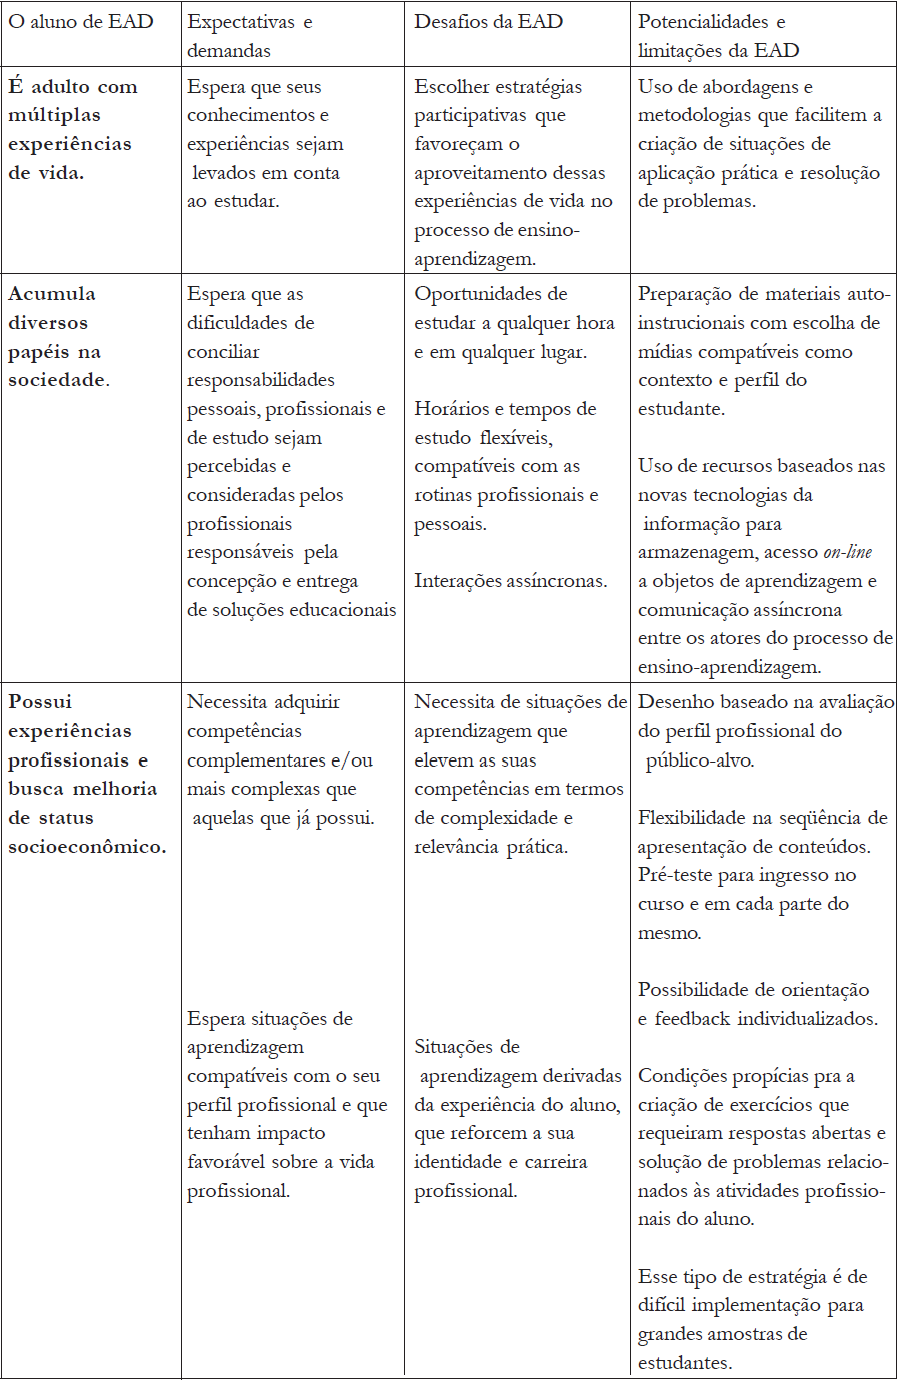
\includegraphics[width=0.9\textwidth]{Tabela_EAD_1_Abbad_2007.png}
            \end{center}
            \caption{A Clientela de EAD (Abbad 2007\cite{Abbad_2007})}
            \label{fig:Clientella_EAD_1}
\end{figure}

  

\begin{figure}
            \begin{center}
                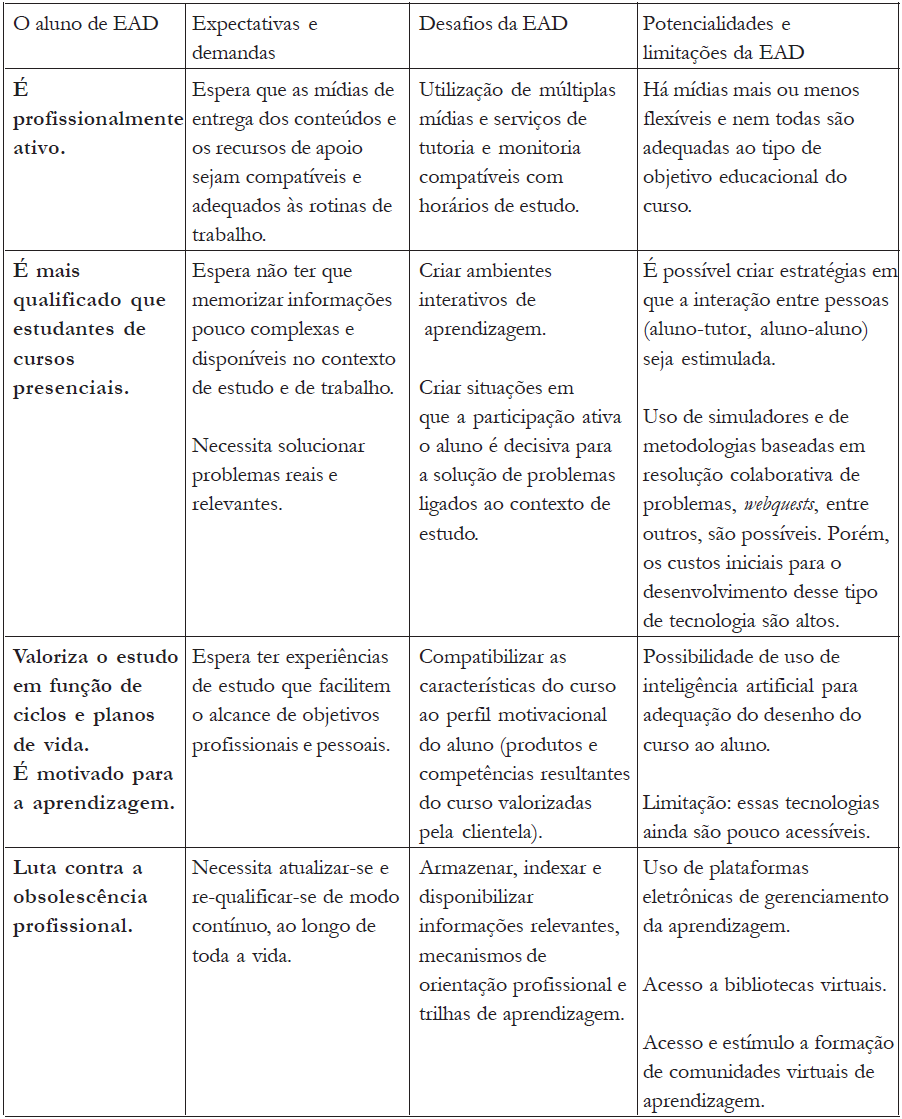
\includegraphics[width=0.9\textwidth]{Tabela_EAD_2_Abbad_2007.png}
            \end{center}
            \caption{A Clientela de EAD (continuação) (Abbad 2007\cite{Abbad_2007})}
            \label{fig:Clientella_EAD_1}
\end{figure}

Além das iniciativas públicas, voltadas a democratização do acesso a educação e a competitividade mercadológica a nível nacional, a realidade atual do mercado globalizado, intensamente dependente das tecnologias da informação e com alta velocidade de evolução, não deixa dúvida sobre a importância da educação continuada para as organizações privadas. Seja para permitir maior produtividade, seja como atrativo para evitar a evasão de mão de obra qualificada, muitas empresas reconheceram a necessidade de providenciar a seus funcionários oportunidades de estudo para manter sua competitividade no mercado globalizado atual. Em vista da complexidade do processo educativo, e de seu alto custo, a eficácia e a eficiência tornam-se preocupações centrais. A partir da década de 50, nos Estados Unidos, empresas de grande porte começaram a implementar Universidades Corporativas de maneira a centralizar seus processos de treinamento (Freitas-Dias e Albuquerque, 2014\cite{Freitas_Albuquerque_2014}, permitindo maior controle sobre o processo educativo. Jeanne Meister (1999 \cite{Meister_1999}, ) define Universidade corporativa como "um guarda-chuva estratégico para desenvolver e educar  funcionários, clientes, fornecedores e comunidade, a fim de cumprir as estratégias empresariais da organização". Vergara (2000 \cite{Vergara_2000}, apud Freitas-Dias e Albuquerque, 2014 \cite{Freitas_Albuquerque_2014}) destaca a importância das universidades corporativas na criação e manutenção da base de conhecimento da empresa, e salienta o ganho em eficiência devido a criação de um código comum de referência para a empresa, seus colaboradores, e seus clientes.Allen (2002 \cite{Allen_2002}, apud Freitas-Dias e Albuquerque, 2014 \cite{Freitas_Albuquerque_2014})descreve a universidade corporativa como uma ferramenta estratégica criada com o objetivo de auxiliar a organização a alcançar sua missão, e Eboli (2002 \cite{Eboli_2002}, apud Freitas-Dias e Albuquerque, 2014 \cite{Freitas_Albuquerque_2014}) ressalta o foco em identificar e desenvolver as competências críticas a busca dos resultados de uma empresa, alem de apresentar o principio de perpetuidade, referindo-se ao papel da educação corporativa na consolidação, fortalecimento e disseminação da cultura organizacional (2004 \cite{Eboli_2004}, apud Freitas-Dias e Albuquerque, 2014 \cite{Freitas_Albuquerque_2014})
Apesar do publico alvo de tais universidades corporativas constituir-se principalmente de adultos, empregados e com experiência nas áreas de conhecimento utilizadas na pratica comercial das empresas, apresentando grande correlação com as características clássicas dos alunos da educação a distância, estas instituições apresentam certa resistência a implementação de cursos nesta modalidade. Albertim e Brauer (2012 \cite{Albertin_Brauer_2012}) apresentam e validam um modelo teórico das causas de tal resistência, baseado no modelo de Teoria Unificada de Aceitação e Uso da Tecnologia (Utaut), elaborado e validado por Venkatesh e colaboradores em 2003. Neste modelo, os autores apresentam os seguintes construtos:

Expectativa de esforço: grau de facilidade associado ao uso do sistema.

Condições Facilitadoras: Grau em que um funcionário acredita que existe uma infraestrutura organizacional e técnica para suportar o uso do sistema.

Interatividade: Grau de interatividade e tempestividade entre o funcionário aluno e o tutor ou com outros alunos.

Expectativa de desempenho: Grau em que um funcionário acredita que o uso do sistema vai ajudá-lo a atingir ganhos no trabalho.

Autoeficácia: Grau de habilidade do funcionário em aprender sozinho e em realizar o que planeja.

Resistência à EAD na EC: Grau em que o funcionário resiste à EAD

No modelo apresentado, a resistência a cursos na modalidade Educação a distância na Educação Corporativa é diretamente influenciada, com correlação negativa, ao grau de Autoeficácia e à expectativa de desempenho do aluno, e indiretamente influenciada, a través da expectativa de desempenho, pela expectativa de esforço do aluno, com correlação positiva, e pelas condições facilitadoras e pelo grau de interatividade esperado do curso, com correlações negativas.

\begin{figure}
            \begin{center}
                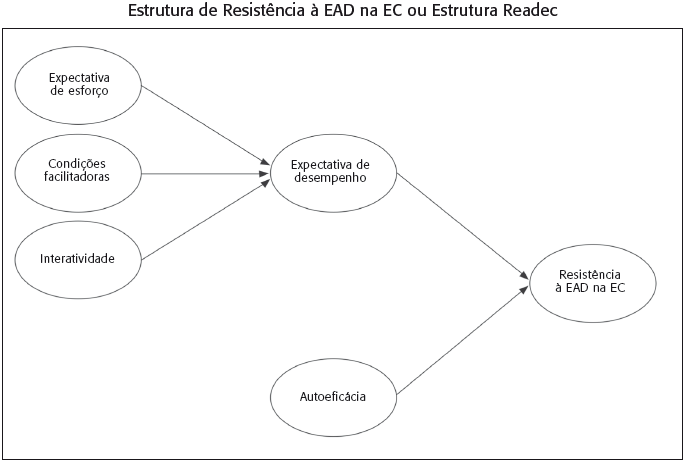
\includegraphics[width=1\textwidth]{Readec.png}
            \end{center}
            \caption{Estrutura de resistência à EAD na EC ou Estrutura Readec(Albertim, Brauer, 2012\cite{Albertin_Brauer_2012})}
            \label{fig:Readec}
\end{figure}

Apesar das dificuldades apresentadas, o modelo de Educação a distância continua apresentando bons resultados nos quesitos de escalabilidade, replicabilidade e flexibilidade para os alunos, tornando-o muito desejável para o âmbito das Universidades Corporativas, além de apresentar a possibilidade a empresas de menor porte, sem os recursos para manter tais estruturas, de contrata-los como serviços com maior facilidade, gerando a possibilidade de mitigar parcialmente os altos custos de implementação iniciais das Universidades Corporativas. 

Em seu artigo "As comunidades virtuais como instrumento de educação corporativa: estudo de caso no Tribunal de Contas da União", Mathias e Santos (2014, \cite{Mathias_Santos_2014}) levantam a visão da educação corporativa contínua, não limitada a treinamentos  pontuais, e apresentam as comunidades virtuais  como ferramentas para criar um ambiente de aprendizado contínuo, assim como uma cultura de aprendizado. Os autores apontam a origem do modelo educacional tradicional na sociedade industrial moderna, e seu objetivo de capacitação pontual, posto que as capacidades requeridas neste ambiente possuíam pouca variabilidade ao longo do tempo. Os autores contrastam esta realidade com a sociedade informacional em que estamos inseridos, na qual as demandas de adaptabilidade e aprendizado são elementos centrais da prática profissional em todos os níveis, assim como de todas as áreas de negócios. Consequentemente, os autores apontam a necessidade de adequar as estruturas de aprendizagem para esta nova realidade, voltando o foco dos setores de capacitação profissional da eficiência operacional para a compreensão e respeito ás estratégias organizacionais da empresa, como indica a figura 3.4.

De acordo com os autores, as comunidades virtuais, possibilitadas por Tecnologias Digitais de Informação, Comunicação e Expressão (TDICE) tem sua implantação em ambientes de educação corporativa dificultada principalmente pela resistência de profissionais "imigrantes digitais", ou seja, nascidos ou formados antes da explosão da computação e da Internet, que ainda apresentam resistência ao seu uso intensivo. Os autores indicam que muitos profissionais ainda enxergam ambientes  virtuais de comunicação como espaços "para que os indivíduos possam fazer amigos, trocar fotos, conversar, enfim, interagir sobre aspectos que não pertencem ao ambiente profissional ou educacional." Os autores apresentam como principais vantagens do uso de comunidades virtuais no âmbito da educação corporativa a facilidade de aprendizagem continuada; a possibilidade de discussão  e, consequentemente, inovação sobre os temas abordados; a criação de um repositório comum de conhecimento, facilitando tanto a capacitação de novos funcionários, quanto a aprendizagem de funcionários existentes sobre áreas outras que a sua, facilitando a colaboração entre diferentes áreas de uma empresa; e a disseminação de conhecimento relativo a mudanças. Os autores apontam o uso das TDICEs como recursos de aprendizagem adequados a uma abordagem sociointeracionista da educação, fundamentada pelos estudos desenvolvidos por Vygotsky, Wallon, e Piaget, entre outros, que apontam que o indivíduo aprende pela interação com o outro. 








\begin{figure}
            \begin{center}
                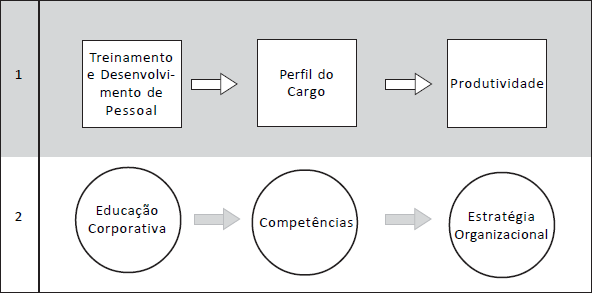
\includegraphics[width=1\textwidth]{Treinamento_v_educacao.png}
            \end{center}
            \caption{Treinamento e educacao(Mathias e Santos, 2014\cite{Mathias_Santos_2014})}
            \label{fig:Treinamento_v_Educacao}
\end{figure}


  %\input{capitulos/capitulo4}
  % ...

  \postextual
  \bibliographystyle{plain}
  \bibliography{bibliografia}

\end{document}
